\section{Design}
	
    \subsection{Aufbau}
    	In diesem Abschnitt wird der Aufbau des Prototypen erklärt. Mann kann sich den Prototypen aufgegliedert in die folgenden drei wesentliche Teile vorstellen:
            
		\begin{description}
			\item[Kivy] ist der Name des verwendeten \emph{frameworks} und vor allem für die Benutzeroberfläche und für das Verarbeiten von Benutzereingaben verantwortlich. Es dient als Rahmen der Applikation und ist für die Kommunikation mit dem jeweiligen Betriebssystem zuständig.
        
        	\item[Learner und Predictor] sind für den \emph{Natural Language Processing} Teil der Anwendung zuständig. Der \emph{Learner} kann neue Sprachmodelle aus Texten erzeugen. Der \emph{Predictor} kann mit Hilfe dieser Sprachmodelle Wortlisten generieren. 
        
        	\item[Adapter] bilden Signale von verschiedenen Eingabegeräten auf die vom Prototypen definierten Signale ab. Sie ermöglichen es \emph{Plugins} für weitere Eingabegeräte zu schreiben.
		\end{description}
        
        \begin{figure}[H]
			\centering
            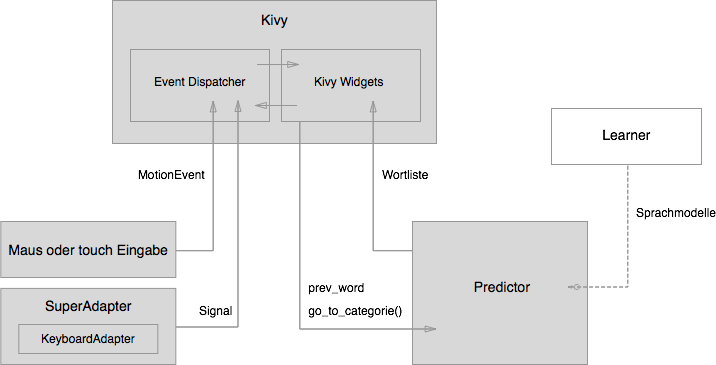
\includegraphics[width=.8\linewidth]{images/aufbau.png}
            \caption{Aufbau des Prototypen}
            \label{fig:architecture}
        \end{figure}
    
    \newpage
	\subsection{Kivy}
    	Die Software ist in \emph{Python} geschrieben. \emph{Python} scheint eine viel für \emph{Natural Language Processing} verwendete Sprache zu sein. Sucht man z. B. auf \emph{github.com} nach den in \autoref{tab:githubNLP} gezeigten Begriffen, liegt Python als Sprache immer weit vorne.
        
        \begin{figure}[H]
			\centering
                
			\begin{tabular}{ r || c | c | c}
                \diagbox{Sprache}{Suchbegriff} & NLP & Natural Language & Natural Language Processing \\ \hline \hline
                Python & 1168 & 500 & 348\\ \hline
                Java & 740 & 269 & 172\\ \hline
                JavaScript & 135 & 146 & 37 \\ \hline
                Ruby & 103 & 100 & 28 \\ \hline
                C++ & 76  & 45 & 23 \\ \hline
            \end{tabular}
            \caption{Anzahl gefundener Repositories in den top fünf Sprachen für die entsprechenden Suchbegriffe auf \texttt{https://github.com/search} (besucht am 02.07.2015)}
			\label{tab:githubNLP}
		\end{figure}
        
        Für \emph{Python} gibt es viele verschiedene \emph{frameworks} zur Erstellung von grafischen Benutzeroberflächen. Eine Liste davon findet sich unter \texttt{https://wiki.python.org/moin/GuiProgramming}.
        
        Für den Prototypen wird ein \emph{open source framework} mit dem Namen \emph{Kivy} verwendet. Laut der Offiziellen Webseite \parencite{kivy:homepage} laufen mit \emph{Kivy} geschriebene Aplikationen unter Linux, Windows, OS X, Android und iOS. Dazu muss die Applikation für jedes entsprechnende System gepackt werden.
        
		Wie in der Dokumentation unter \cite{kivy:events} beschrieben wird, fasst \emph{Kivy} verschiedene \emph{Input events} als \texttt{MogtionEvent} zusammen. Für einen Button macht es keinen Unterschied, ob er mit einer Maus geklickt oder mit dem Finger gedrückt wurde.
        
        \emph{Kivy} stellt auch eine eigene \texttt{EventDispatcher} Klasse zur verfügung. Diese steuert die Signale von \emph{touch}- oder Mauseingaben, sowie Signale, die von den \emph{Adaptern} gesendet werden. Eine \emph{Kivy} Applikation besteht aus sogenannten \emph{widgets}. Wie in der Dokumentation unter \cite{kivy:widgets} erklärt, hat ein \emph{widget} einen \emph{Canvas} in welchen gezeichnet werden kann. Es kann auf \emph{events} reagieren und diese selbst senden. \emph{Widgets} sind als \emph{tree} organisiert und jede Applikation benötigt zumindest ein \emph{root widget}
        
        Im \emph{root widget} des Prototypen befinden sich \emph{handler} für die Signale, die von den \emph{Adaptern} gesendet werden können. Außerdem wird hier eine Instanz des \texttt{WordPredictor}s erzeugt, von welcher Kategorien und Wortlisten generiert werden. Dazu wird dem \texttt{WordPredictor} durch einen Aufruf von \texttt{go\_to\_categorie()} die von Nutzer gewählte Kategorie mitgeteilt. Und nach jeder Wortauswahl wird das ausgewählte Wort \texttt{prev\_word} an den \texttt{WordPredictor} gesendet. Siehe \autoref{fig:architecture}.
        
    \newpage
	\subsection{Learner und Predictor}
    \label{sec:design-learnerPredictor}
    
    	Der \emph{Learner} besteht aus zwei speraten Teilen. Aus einem \emph{Tokenizer} und einem \emph{Clusterer}. Der \emph{Tokenizer} hat die Aufgabe, Texte wie sie z.B. in einem Buch zu finden sind, zu bereinigen. Dem \emph{Tokenizer} werden mehrere Textdateien übergeben aus welcher dieser eine einzelne neue Textdatei generiert. Darin befindet sich der bereinigte Text in einer Form wie er von dem \emph{Clusterer} gelesen werden kann.

		Der \emph{Clusterer} liest und analysiert die vom \emph{Tokenizer} generierte Textdatei. Dieser Umweg über eine extra generierte Datei ist nötig, da für den \emph{Clusterer} eine \emph{third party} Lösung verwendet wird. Dies wird in \autoref{sec:thirdTry} genauer beschrieben. In erster Linie gruppiert der \emph{Clusterer} die übergebenen Worte in Klassen und speichert das Ergebniss wieder in mehreren Dateien ab. Diese Dateien enthalten neben den Worklassen auch die Information wie oft ein bestimmtes Wort nach einem anderen kommt. Die vom \emph{Clusterer} generierten Dateien werden im folgenden \emph{Sprachmodell} genannt.

		Das generieren von \emph{Sprachmodellen} ist nicht Teil der gepackten Applikation. Dazu muss für jedes neue Sprachmodell der \emph{Tokenizer} und der \emph{Clusterer} von Hand aufgerufen werden. Das generierte \emph{Sprachmodell} wird dann in den dafür vorgesehen Ordner in der Applikation gelegt.

		In der laufenden Applikation kann der Nutzer eine Kategorie auswählen. Diese entspricht immer einem \emph{Sprachmodell}. Nach der Auswahl wird wird dieses automatisch von dem \emph{Predictor} geladen. Dieser Prozess wird in \autoref{sec:implemetation-wordPredition} genauer beschrieben. Aufgrund des Sprachmodells wird vom \emph{Predictor} dann eine Wortliste generiert.
       
    \newpage
    \subsection{Adapter}
    	Wie in \autoref{sec:requirements-input} gefordert ist es möglich die Applikation ausschließlich mit den drei Signalen \texttt{left}, \texttt{right} und \texttt{enter} zu bedienen. Abgesehen von der Eingabe per \emph{touch} oder mit der Maus reagiert die Applikation nicht direkt auf Eingaben von z. B. der Tastatur sondern nur auf die in \texttt{SuperAdapter} beschriebenen Signale.  
    
    	Ein \emph{Adapter} besteht aus einer einzigen \emph{Python} Datei mit dem Namen des Gerätes, für das er geschrieben wurde, kombiniert mit dem Wort \emph{Adapter}. Jeder \emph{Adapter} muss von der Klasse \texttt{SuperAdaper} erben. \texttt{SuperAdaper} wiederum erbt von \emph{Kivy}'s \texttt{EventDispatcher}.
So ist es einfach innerhalb der Applikation auf Signale zu reagieren. Ein \emph{Adapter} muss der Applikation mitteilen können ob das dazugehörige Gerät verfügbar ist. Sollte das nicht der Fall sein wird ein \emph{Adapter} nicht geladen.

		Des weiteren muss ein \emph{Adapter} minnimal die drei Signale \texttt{left}, \texttt{right} und \texttt{enter} senden können. Wenn möglich kann ein Adapter auch noch weitere Signale senden. Mögliche weitere Signale sind: \texttt{up}, \texttt{down}, \texttt{talk} und \texttt{close}.
        
        Jeder neue \emph{Adapter} muss in dem Ordner \texttt{inputAdapters} gespeichert werden. Außerdem muss dieser in der \texttt{\_\_init\_\_.py} im gleichen Ordner importiert und in die Liste \texttt{adapters} eingetragen werden. Durch diesen Prozess wird erreicht, dass für das Hinzufügen von einem \emph{Adapter} nur Änderungen innerhalb eines einzigen Ordners vorgenommen werden müssen. Adapter leben also getrennt von der Applikation in einem eigenen Modul. Um einen Adapter zu schreiben müssen lediglich die oben gennanten Anforderungen eingehalten werden. Es sind keine weiterem Kenntnisse über die interne Funktionsweise des Prototypen nötig. Ein System zum einbinden von externen Adaptern in eine gepackte Applikation existiert allerdings nicht.
	
    \newpage